\documentclass[aspectratio=169,usenames,dvipsnames]{beamer}
\beamertemplatenavigationsymbolsempty
% \documentclass{beamer}

% UNCOMMENT FOR HANDOUTS
% \usepackage{pgfpages}
% \pgfpagesuselayout{2 on 1}[landscape,letterpaper,border shrink=5mm]
% \setbeameroption{show notes}

\mode<presentation>
\usetheme{Boadilla}
\usecolortheme{spruce}
\usepackage{../../LizStyle,ulem}
\usepackage{color}
\usepackage[color,matrix,arrow]{xy}
% \input xy
% \xyoption{all}
\usepackage{tikz}
\usepackage{tikz-cd}
\tikzset{commutative diagrams/diagrams={ampersand replacement=\&}}

\AtBeginSection{\frame{\sectionpage}}


% ==========Command for putting comments and removing them=======
% Visible:
\newcommand{\InstructorNotes}[1]{\textit{\color{orange}#1}}
\newcommand{\InstructorList}[1]{
\begin{itemize}
	\color{orange}
	#1
\end{itemize}
}
\newcommand{\OnlyStudent}[1]{}
% Removed:
 \renewcommand{\InstructorNotes}[1]{}
\renewcommand{\InstructorList}[1]{}
% \renewcommand{\OnlyStudent}[1]{#1}



\newcommand{\bvfill}{\vskip0pt plus 1filll}

\usepackage{multimedia}
\usepackage{graphbox}

% \usepackage{algpseudocode}


\newcommand{\Reeb}{\textbf{Reeb}}
\newcommand{\Rtopc}{\textbf{Rtopc}}
% \newcommand{\RR}{\mathcal{R}}

\newcommand{\Set}{\textbf{Set}}
\newcommand{\Vect}{\textbf{Vect}}
\newcommand{\Top}{\textbf{Top}}
\newcommand{\Int}{\textbf{Int}}


\graphicspath{ {Figures/} {../Figures/}{../../Figures/} }



\begin{document}
%\pdfoptionpdfminorversion 5
%\logo{\includegraphics[height=1.5cm]{dukeshield.pdf}}
\title[]{Ch 9.1: Maximum Margin Classifier }
\subtitle{Lecture 26 - CMSE 381}
\date{Mon, Mar 30, 2026}



\institute[MSU-CMSE]{Michigan State University\\
			::\\
          Dept of Computational Mathematics, Science \& Engineering}
%\author[Dr.~Zhang]{Prof.~Mengsen Zhang}

\begin{frame}
 \titlepage


\end{frame}
%--------------------------
\begin{frame}[c]{Announcements }

\begin{columns}
\column{.45\textwidth}
\centering

	\textbf{Last time:}
	\begin{itemize}
	\item Ch 8: Random Forests
	\end{itemize}

	\vspace{.2in}

	\textbf{This lecture:}
	\begin{itemize}
	\item Maximal Margin Classifier
	\item No jupyter notebook for this class
\end{itemize}
% \InstructorNotes{Check the example, there are some typos and it tripped me up this time. Edit 2024 - Didn't find it so I think this was from 2 years ago?}
\textbf{Announcements:}
	%\begin{itemize}
	%\item HW \#8 Due Sunday 11/16

	%\end{itemize}


\column{.4\textwidth}
\centering


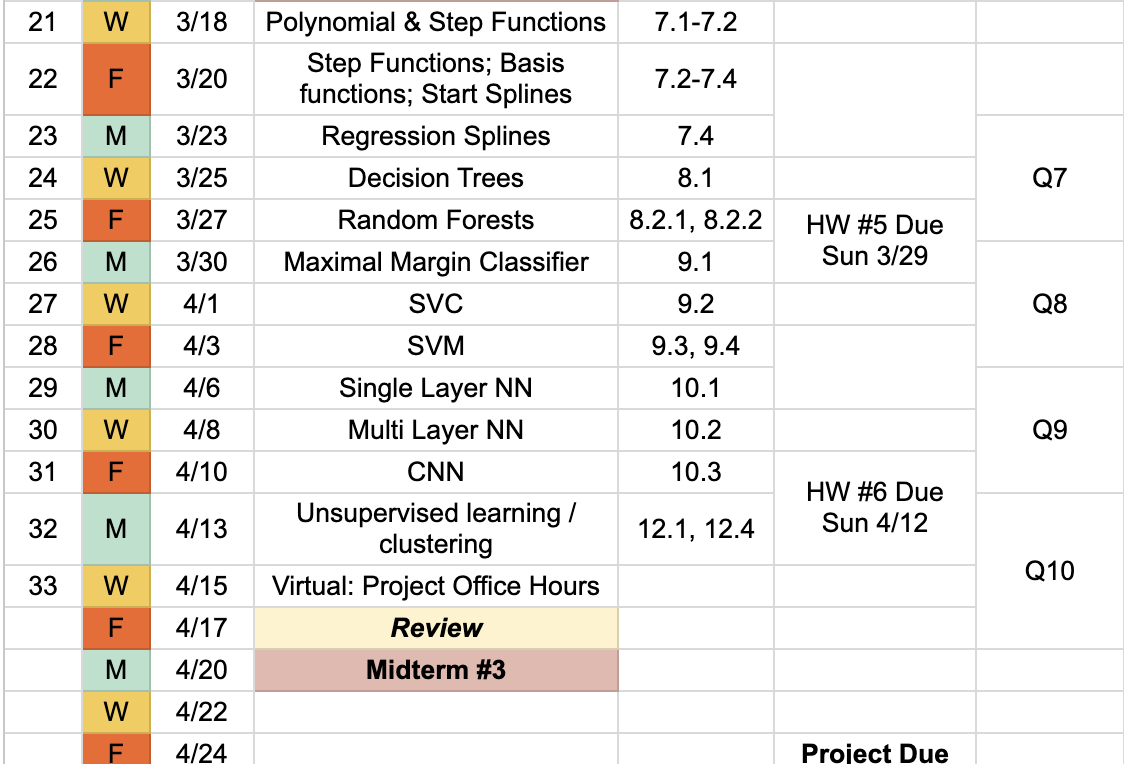
\includegraphics[alt={Screenshot of the course schedule from lectures 21 to 32.}, width = \textwidth]{Schedule-S26-3.png}

\end{columns}

\end{frame}
%--- Next Frame ---%
\begin{frame}[c]{What will you learn today?}

\begin{itemize}
\item What is hyperplane?
	\begin{itemize}
	\item How do you mathematically describe this hyperplane?
	\item How do you mathematically describe the two sides of the hyperplane?
	\item Given the equation of the hyperplane and the coordinates for a point, you should be able to tell which side of the plane the point is on.
	\end{itemize}
\item What qualify a hyperplane as a separating hyperplane?
	\begin{itemize}
	\item You should be able to describe this mathematically using an inequality.
	\item You should also be able to determine whether a hyperplane is a separating hyperplane given a graph, or given the equation of the plane and the coordinates and class of a few points.
	\end{itemize}
\item How to use a separating hyperplane as a classifier?
\item What makes a hyperplane a maximal margin hyperplane?
	\begin{itemize}
	\item What are its margin and support vectors?
	\item Given a graph, you should be able to clearly label the margin and support vectors. You should also be able to infer the size of the margin from reading the graph.
	\item You should also be able to describe the optimization problem mathematically.
	\item Given the equation of the maximal margin hyperplane and the coordinates of support vectors, you should be able to calculate the size of the margin by hand.
	\end{itemize}
\end{itemize}

\end{frame}


%=================
\section{Maximal Margin Classifier}
%=================

% \begin{frame}[t]{The Island of Dr Brain}
% \begin{columns}
% \column{.4\textwidth}
% \centering

% 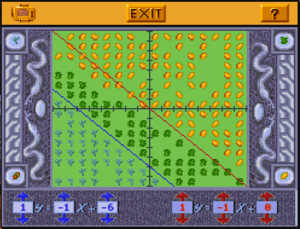
\includegraphics[align = c, width = \textwidth]{300px-Island_of_Dr_Brain_puz2_stan2}
% \column{.4\textwidth}
% \centering
% 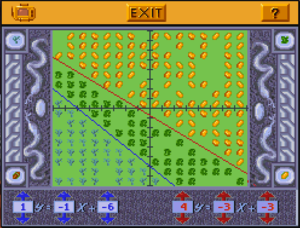
\includegraphics[align = c, width = \textwidth]{300px-Island_of_Dr_Brain_puz2_stan3}
% \end{columns}
% \bvfill
% \url{https://classicreload.com/island_of_dr_brain.html}
% \end{frame}
%--- Next Frame ---%
\begin{frame}[t]{The goal }
\begin{columns}
\column{.45\textwidth}
\centering
\includegraphics[alt={A example of SVM for classification}, width = \textwidth]{SVM-Example}

\column{.45\textwidth}
\centering
\InstructorList{
  \item Point out today is all about classification 
  \item Goal is to find a line in the middle that separates the two classes. Lots of options, but we want the one that stays as far from everyone as possible.
  \item For today, need to use $y \in \{ -1,1\}$ for this to make sense.
}

\end{columns}
\end{frame}
%--- Next Frame ---%

\begin{frame}[t]{What is a hyperplane?}

\begin{columns}
\column{.45\textwidth}
\centering
\InstructorList{
  \item In $p$-dimensional space, a hyperplane is a flat affine subspace of dimension $p-1$
  \item affine means it doesn't have to pass through the origin
	\item Draw example for $p=1,2,3$
}


\column{.45\textwidth}
\centering

\end{columns}

\end{frame}
%--- Next Frame ---%
\begin{frame}[t]{Mathematical definition of a hyperplane}

	\begin{equation*}
		\beta_0 + \beta_1X_1 + \beta_2X_2 + \cdots + \beta_p X_p = 0
	\end{equation*}

\begin{columns}
\column{.45\textwidth}
\centering
\InstructorList{
  \item Being on the hyper plane means having a point $X=(X_1,X_2,\cdots,X_p)^T$ satisfying this
	\item Show that when $p=2$, this is just a line
}

\column{.45\textwidth}
\centering

\end{columns}

\end{frame}
%--- Next Frame ---%

\begin{frame}[t]{Hyperplane for $p=2$}

\begin{columns}
\column{.45\textwidth}
\centering
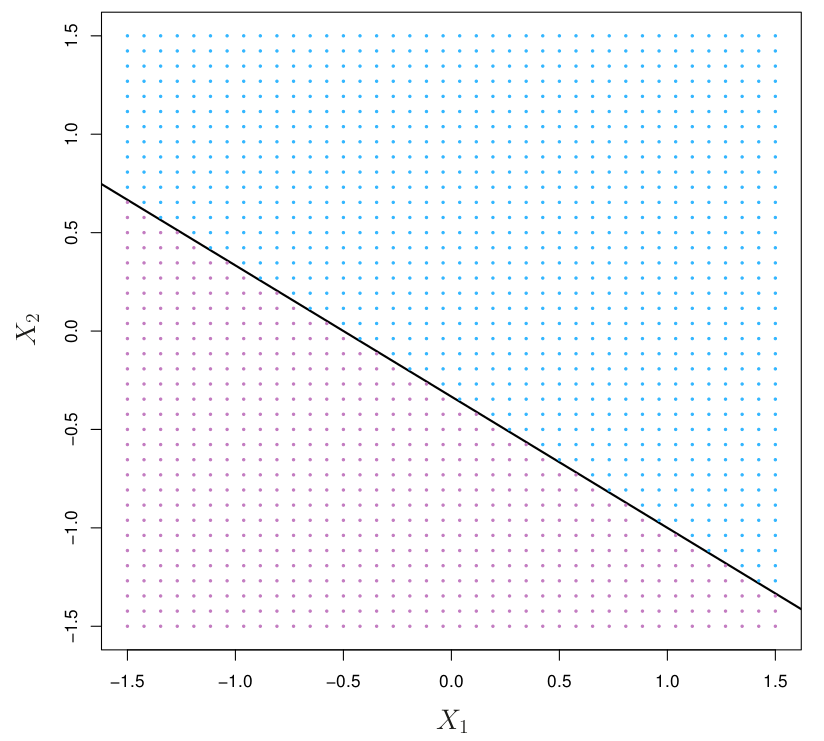
\includegraphics[alt={A hyperplane separate two regions with blue and purple colors. }, width = \textwidth, align = c]{Fig9-1}
$1+2X_1 + 3X_2 = 0$
\column{.45\textwidth}
\InstructorList{
	\item point of some examples:
	\item $X_1=-0.5$, $X_2=0$
	\item $X_1=0$, $X_2=-1$ , on lower left with $1+2X_1 + 3X_2 < 0$
	\item $X_1=0$, $X_2=1$ , on upper right with $1+2X_1 + 3X_2 > 0$
}
\centering

\end{columns}

\end{frame}
%--- Next Frame ---%
\begin{frame}[t]{There are two sides to every hyperplane}

\begin{columns}
\column{.45\textwidth}
\centering
\begin{equation*}
		\beta_0 + \beta_1X_1 + \beta_2X_2 + \cdots + \beta_p X_p < 0
\end{equation*}
\column{.45\textwidth}
\centering
\begin{equation*}
		\beta_0 + \beta_1X_1 + \beta_2X_2 + \cdots + \beta_p X_p > 0
\end{equation*}
\end{columns}
\bvfill
\centering
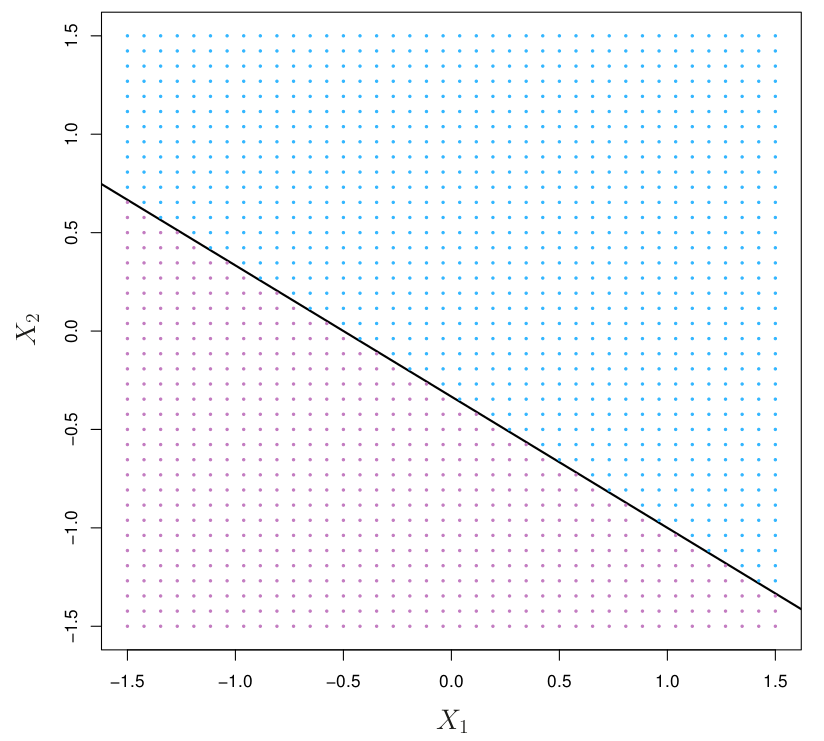
\includegraphics[alt={A hyperplane separate two regions with blue and purple colors. }, width = .4\textwidth, align = c]{Fig9-1}

\end{frame}
%--- Next Frame ---%


\begin{frame}[t]{Classification Setup}

\begin{columns}
\column{.45\textwidth}
\centering
 Data matrix:
	\begin{equation*}
		X =
		\begin{pmatrix}
			- & x_1^T & -\\
			- & x_2^T & -\\
			 & \vdots & \\
			- & x_n^T & -
		\end{pmatrix}_{n \times p}
	\end{equation*}

	\begin{equation*}
		x_1 =
		\begin{pmatrix}
			x_{11} \\
			\vdots \\
			x_{1p}
		\end{pmatrix}
		,\cdots,
		x_n =
		\begin{pmatrix}
			x_{n1} \\
			\vdots \\
			x_{np}
		\end{pmatrix}
	\end{equation*}

\column{.45\textwidth}
\centering
 Observations in one of two classes, $y_i \in \{-1,1\}$
	\begin{equation*}
		Y =
		\begin{pmatrix}
			y_1 \\
			y_2\\
			\vdots \\
			y_n
		\end{pmatrix}
	\end{equation*}


% \column{.4\textwidth}
% \centering

\end{columns}
\bvfill
\centering
Separate out a test observation
\begin{equation*}
	x^* = (x_1^* \; \cdots \; x^*_p)^T
\end{equation*}
\end{frame}
%--- Next Frame ---%


\begin{frame}[t]{Separating Hyperplane}

\vspace{-.2in}
\begin{align*}
	\beta_0 + \beta_1x_{i1} + \beta_2 x_{i2} + \cdots + \beta_px_{ip} >0 \text{ if } y_i & = 1\\
	\beta_0 + \beta_1x_{i1} + \beta_2 x_{i2} + \cdots + \beta_px_{ip} <0 \text{ if } y_i & = -1\\
\end{align*}
\vspace{-.4in}
\begin{columns}
\column{.4\textwidth}
\centering
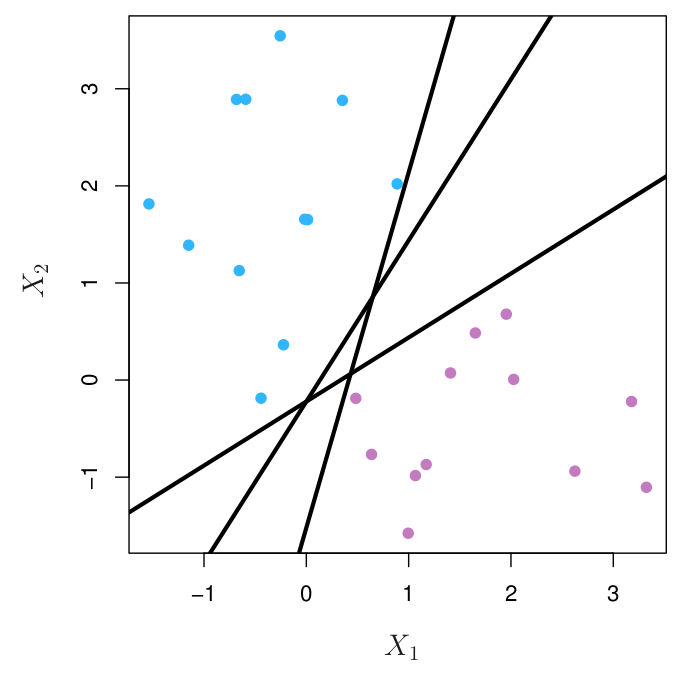
\includegraphics[alt={Three separating hyperplanes separate for two classes of observations. },width = \textwidth, align = c]{Fig9-2a}
\column{.45\textwidth}
\centering
\InstructorList{
  \item Strict requirement
	\item No points can be on the wrong side of the line
}

\end{columns}

\end{frame}
%--- Next Frame ---%
\begin{frame}[t]{Another way to say it}

\begin{align*}
	\beta_0 + \beta_1x_{i1} + \beta_2 x_{i2} + \cdots + \beta_px_{ip} >0 \text{ if } y_i & = 1\\
	\beta_0 + \beta_1x_{i1} + \beta_2 x_{i2} + \cdots + \beta_px_{ip} <0 \text{ if } y_i & = -1\\
\end{align*}

\bvfill
\centering
For all $i$:
\begin{equation*}
	y_i(\beta_0 + \beta_1x_{i1} + \beta_2 x_{i2} + \cdots + \beta_px_{ip}) > 0
\end{equation*}
\bvfill

\end{frame}
%--- Next Frame ---%
\begin{frame}[t]{Separating hyperplane becomes a classifier }

\begin{columns}
\column{.45\textwidth}
\centering
If you have a separating hyperplane:
\begin{itemize}
	\item Check
	\begin{equation*}
		f(x^*) = \beta_0 + \beta_1x_{1}^* + \beta_2 x_{2}^* + \cdots + \beta_px_{p}^*
	\end{equation*}
	\item If positive, assign $\hat y = 1$
	\item If negative, assign $\hat y = -1$
\end{itemize}
\column{.45\textwidth}
\centering
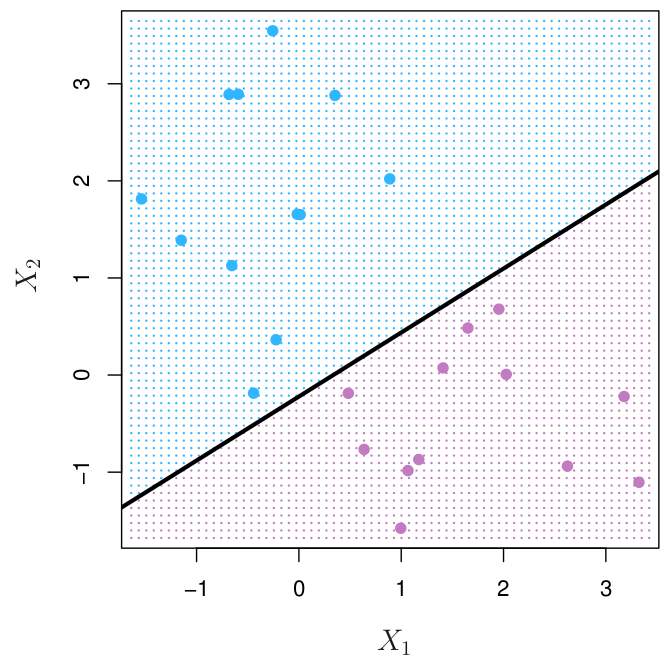
\includegraphics[alt={A separating hyperplane becomes a classifier }, width = \textwidth, align = c]{Fig9-2b}
\end{columns}

\end{frame}
%--- Next Frame ---%
\begin{frame}[t]{How do we pick?}

\begin{columns}
\column{.45\textwidth}
\centering
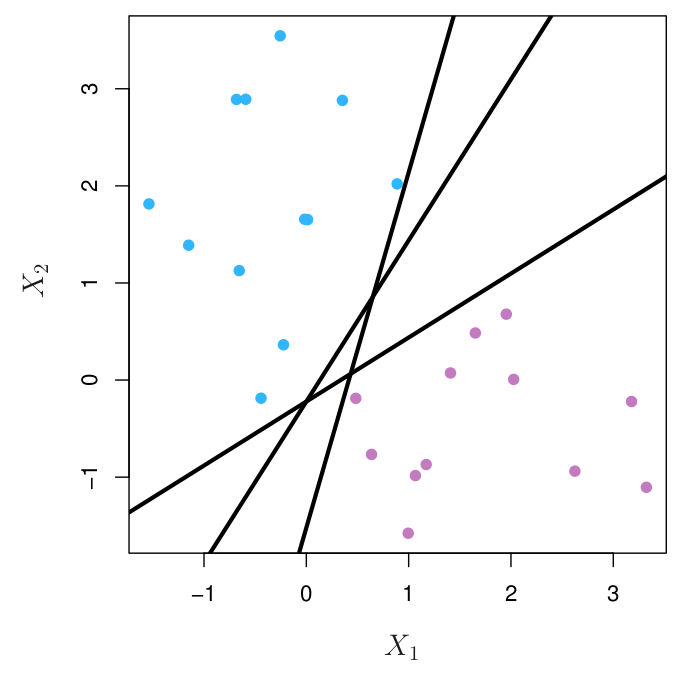
\includegraphics[alt={Three separating hyperplanes separate for two classes of observations. },width = \textwidth, align = c]{Fig9-2a}
\column{.45\textwidth}
\centering
\InstructorList{
  \item
\InstructorNotes{There's lots of separating hyperplanes here, so how do we find a "best" one?}
\item Compute the perpendicular distance from each training observation to a given separating hyperplane
\item Smallest such distance is the \textit{margin}
}

\end{columns}

\end{frame}
%--- Next Frame ---%
\begin{frame}[t]{Distance from an observation to a hyperplane}
\begin{columns}
\column{.4\textwidth}
\centering
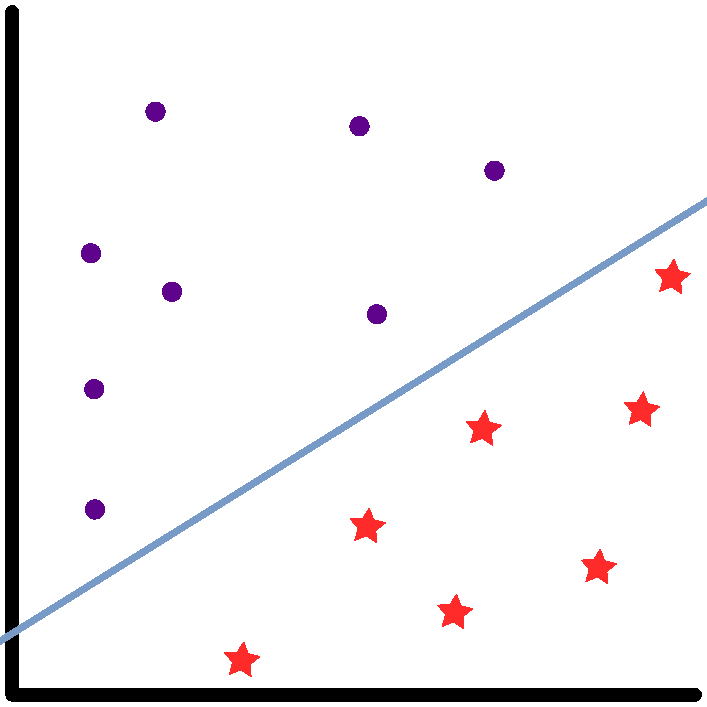
\includegraphics[alt={SVM example with line 1 },align = c, width = \textwidth]{SVM-example-WithLine1}

\column{.4\textwidth}
\centering
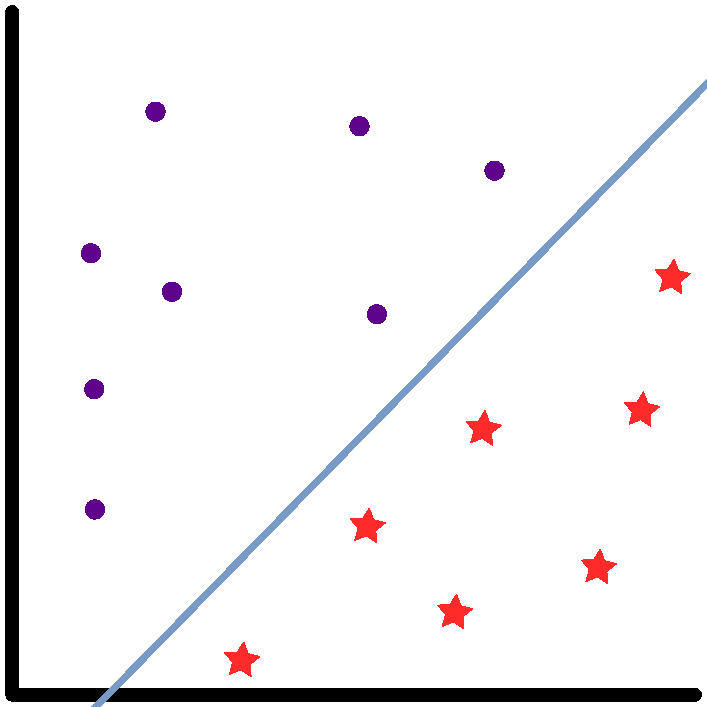
\includegraphics[alt={SVM example with line 2 },align = c, width = \textwidth]{SVM-example-WithLine2}
\end{columns}
\end{frame}
%--- Next Frame ---%
\begin{frame}[t]{Maximal margin classifier}

\begin{columns}
\column{.45\textwidth}
\centering
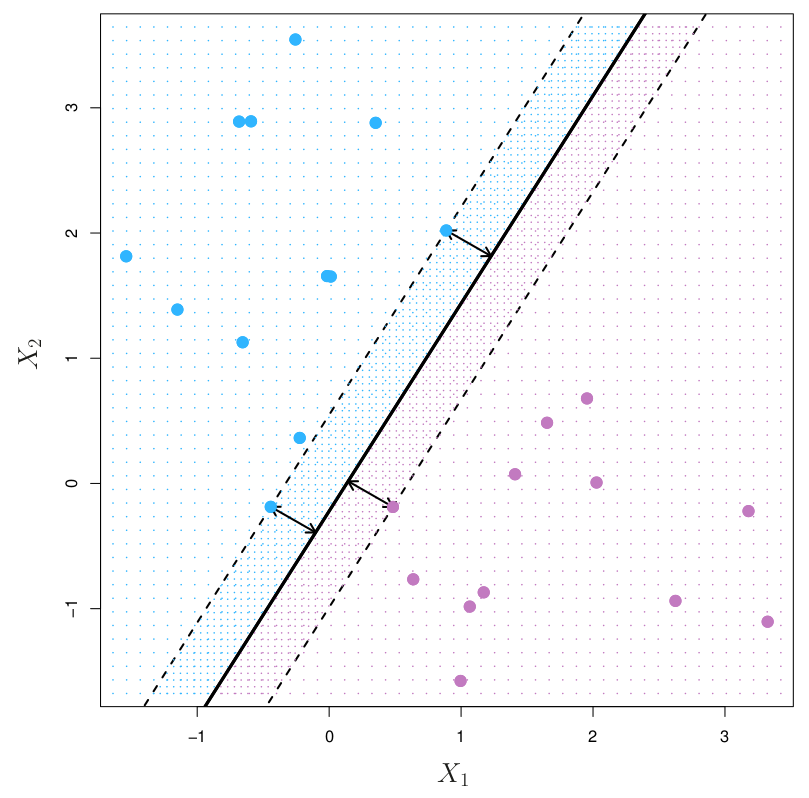
\includegraphics[width = \textwidth, align = c]{Fig9-3}
\column{.45\textwidth}
\centering
\InstructorList{
\item \textit{Maximal margin hyperplane} is the hyperplane with the largest minimum distance to the training observations
\item Classify using it gives you the \textit{maximal margin classifier}
\item Observations that are closest are called \textit{support vectors}
\item If points moved slightly then MMH would move
\item No effect if any other points moved
}

\end{columns}

\end{frame}
%--- Next Frame ---%
{
\setbeamercolor{background canvas}{bg=Apricot!25}
\begin{frame}[t]{Example}
\begin{columns}
\column{.45\textwidth}
\centering
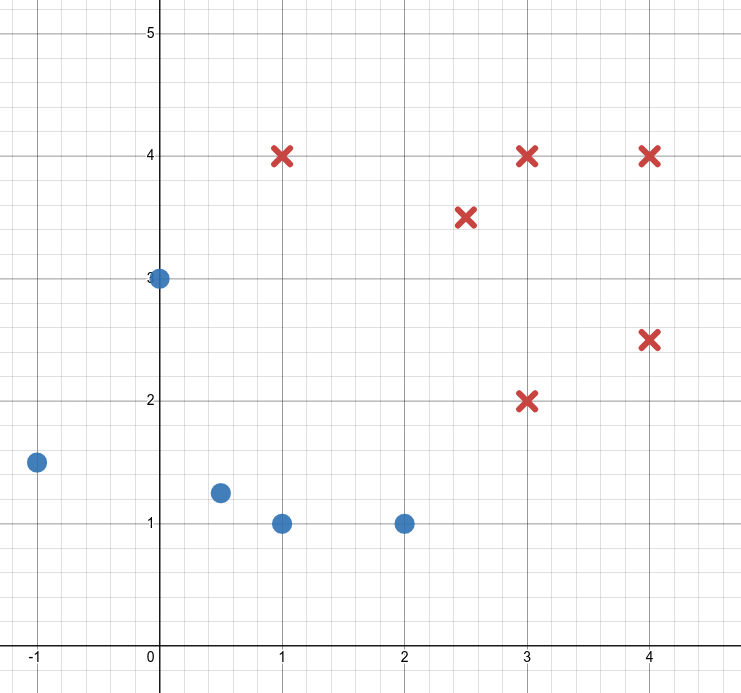
\includegraphics[align = c, width = \textwidth]{SVM-DesmosExample}

\column{.45\textwidth}
\centering
\begin{itemize}
	\item Sketch the maximal margin hyperplane. 
	\item What is the equation of this line in the form $\beta_0 + \beta_1X_1 + \beta_2 X_2 = 0$? 
	\item Circle the support vectors. What is their distance from the line?
	% \item Which side of the line has $\beta_0 + \beta_1X_1 + \beta_2 X_2 > 0$
\end{itemize}
\end{columns}

\bvfill
\url{https://www.desmos.com/calculator/tklbommiwz}
\end{frame}
}
%--- Next Frame ---%
{
\setbeamercolor{background canvas}{bg=Apricot!25}
\begin{frame}[t]{Extra work space}
\begin{columns}
\column{.45\textwidth}
\centering
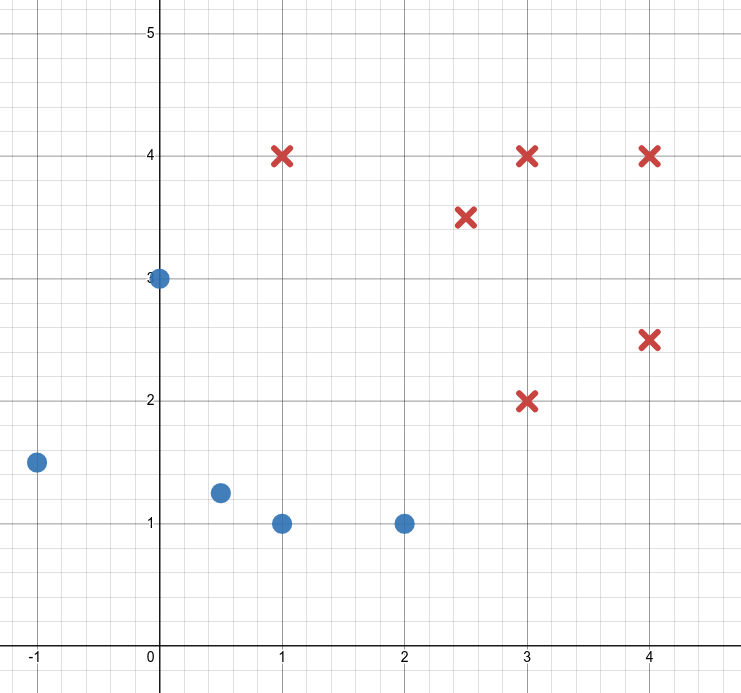
\includegraphics[align = c, width = \textwidth]{SVM-DesmosExample}

\column{.45\textwidth}
\centering
Respond to \href{https://PollEv.com/multiple_choice_polls/2q6UsD3rYTqB3c0z2IiNF/respond}{PollEv question}.

\InstructorList{
  \item $X_1 + X_2- 4 = 0 $
  \item test points $(0,0)$, $(4,4)$, $(2,2)$
  \item Points are at distance $\frac{\sqrt{2}}{2}$. Build the isoceles right triangle with $d$ on two sides and 1 for hypotenuse.

}


\end{columns}

\bvfill
\url{https://www.desmos.com/calculator/tklbommiwz}
\end{frame}
}
%--- Next Frame ---%

\begin{frame}[t]{Mathematical Formulation}

\begin{columns}
\column{.65\textwidth}
\centering
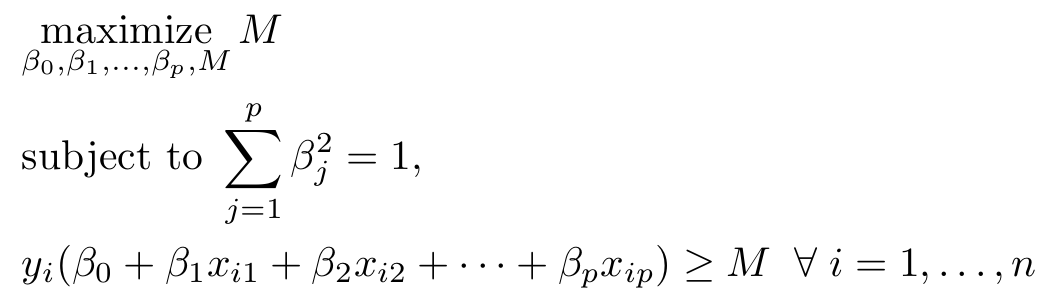
\includegraphics[width = \textwidth, align = c]{Eq9-9}
\column{.35\textwidth}
\centering
\InstructorList{
  \item Last eq forces points to be on the correct side of the hyperplane if $M>0$
	\item Making $M$ as big as possible is the maximal margin hyperplane
}

\end{columns}

\end{frame}
%--- Next Frame ---%


\begin{frame}[t]{First constraint}
	\begin{columns}
	\column{.3\textwidth}
	\centering
	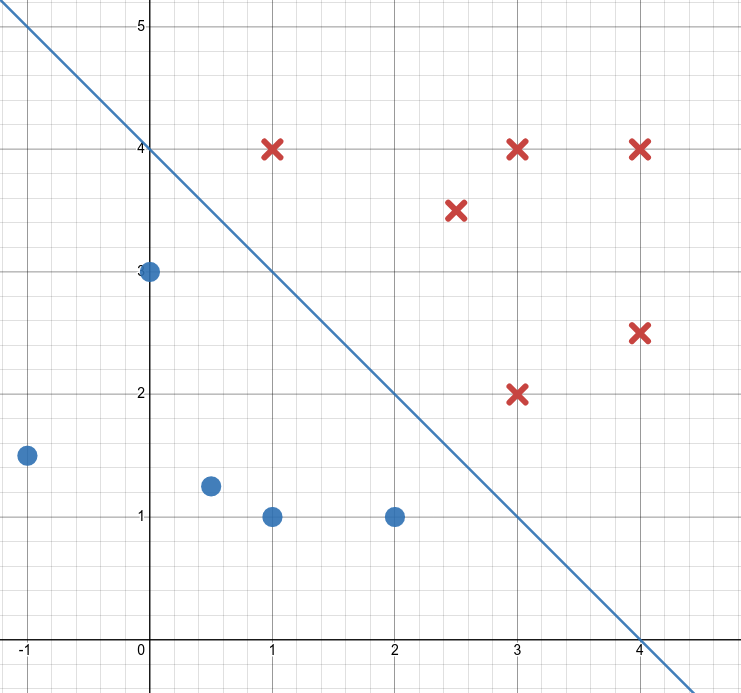
\includegraphics[align = c, width = \textwidth]{SVM-DesmosExample-WithLine}
	
	\column{.65\textwidth}
	\centering
	\InstructorList{
	  \item Had the equation $-4 + X_1 + X_2  = 0 $
	  \item Can divde by any number and get the same line.
	  \item $\sum_{i=1}^p \beta_i^2 = 1^2 + 1^2 = 2$
	  \item We get the same sloped line if we divide by $\sqrt{\left(\sum \beta_i\right)}$, 
	  \item Just need to solve for the intercept
	  \item $-\frac{4}{\sqrt 2}+\frac{1}{\sqrt 2} X_1 + \frac{1}{\sqrt 2} X_1 	   = 0$
	  \item $-2 \sqrt 2+\frac{\sqrt 2}{2} X_1 + \frac{\sqrt 2}{2} X_1 = 0$
	  \item Check that $\sum_{i=1}^p \beta_i^2$ is now 1
	  \item plug in the support vector $x_i=(1,4)$, which give $y_i(\beta_0+\beta_1X_{i1}+\beta_2X_{i2})=1/\sqrt{2}=:M$ (the margin)
	  \item Note that $y = 1$ is Red X, $y = -1$ is blue dots below the line
	}
	
	\end{columns}
	\end{frame}
	%--- Next Frame ---%

	\begin{frame}[t]{Second constraint}
	
	\begin{columns}
		\column{.35\textwidth}
	\centering
	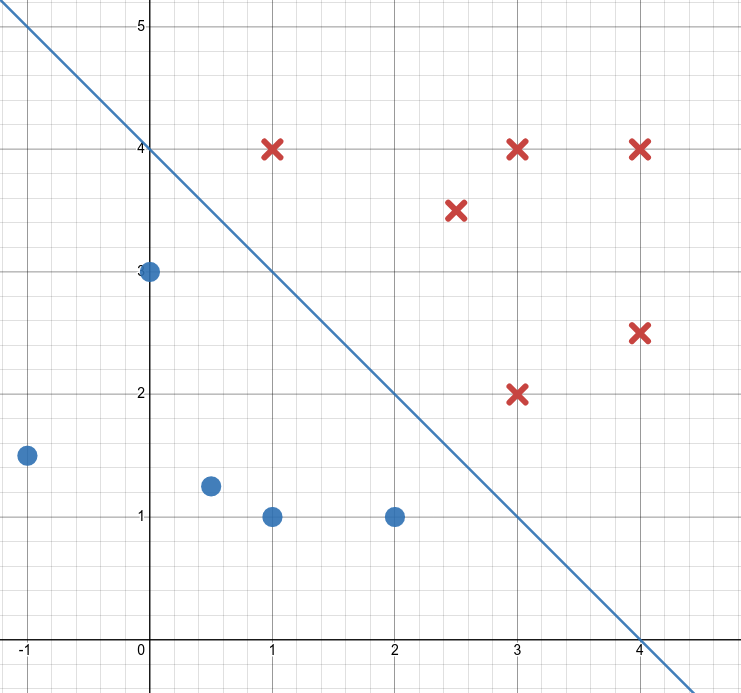
\includegraphics[align = c, width = \textwidth]{SVM-DesmosExample-WithLine}
	\begin{itemize}
		\item Blue circles: $y_i = -1$ 
		\item Red Xs: $y_i = 1$
		\item $-2 \sqrt 2 + \frac{\sqrt 2}{2} X_1 + \frac{\sqrt 2}{2} X_1 
		 = 0$
	\end{itemize}
	\column{.65\textwidth}
	\centering
	$y_i(\beta_0 + \beta_1 x_{i1} + \beta_2 x_{i2}) \geq M$

	\InstructorList{
	\item For point $(3,2)$: 
	\begin{itemize}
		\item $y_i = 1$ 
		\item $ 1(-2 \sqrt 2 + \frac{\sqrt 2}{2} \cdot 3 + \frac{\sqrt 2}{2} \cdot 2 ) = $ $\frac {\sqrt{2}} {2}$
	\end{itemize}
	  \item For point $(0,3)$: 
	  \begin{itemize}
		\item $y_i = -1$ 
		\item $ -1(-2 \sqrt 2 + \frac{\sqrt 2}{2} \cdot 0 + \frac{\sqrt 2}{2} \cdot 3 ) = $ $\frac {\sqrt{2}} {2}$
	  \end{itemize}
	\item For point $(1,1)$
	\begin{itemize}
		\item $y_i = -1$ 
		\item $ -1(-2 \sqrt 2 + \frac{\sqrt 2}{2} \cdot 1 + \frac{\sqrt 2}{2} \cdot 1 ) = $ ${\sqrt{2}} $
	  \end{itemize}

	}
	

	% Pushes the equation to the top when the instructor stuff isn't here
	\OnlyStudent{\vspace{2.3in}}


	\end{columns}
	\end{frame}
	%--- Next Frame ---%
	{
	\setbeamercolor{background canvas}{bg=Apricot!25}
	\begin{frame}[t]{An example with a bad choice of hyperplane}
	\begin{columns}
	\column{.35\textwidth}
	\centering
	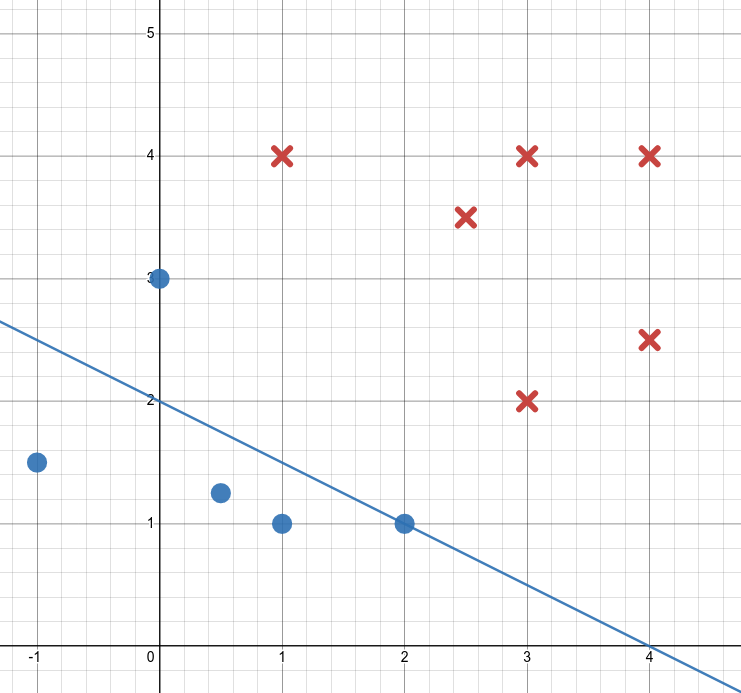
\includegraphics[align = c, width = \textwidth]{SVM-DesmosExample-WithBadLine}
	\begin{itemize}
		\item Blue circles: $y_i = -1$ 
		\item Red Xs: $y_i = 1$
		\item $-\frac{4}{\sqrt{5}} + \frac{1}{\sqrt 5} X_1 + \frac{2}{\sqrt 5} X_1 
		 = 0$
	\end{itemize}
	
	\column{.6\textwidth}
	\centering

	What is $y_i(\beta_0 + \beta_1 x_{i1} + \beta_2 x_{i2})$ for the point $x_i = (0,3)$?
	\InstructorList{
	  \item $-1(-\frac{4}{\sqrt{5}} + \frac{1}{\sqrt 5} \cdot 0 + \frac{2}{\sqrt 5} \cdot 3 )$
	  \item $-1 (-4 + 6) \frac{1}{\sqrt 5}$
	  \item $\frac{-2}{\sqrt 5}$
	  \item Note this is negative, so no positive $M$ will make it so this is a valid line
	}
	

		% Pushes the equation to the top when the instructor stuff isn't here
		\OnlyStudent{\vspace{2.3in}}
		% \vspace{2.3in}
	\end{columns}
	\end{frame}
	}
	%--- Next Frame ---%

	\begin{frame}[t]{Second constraint extra space}
	
		\begin{columns}
			\column{.35\textwidth}
		\centering
		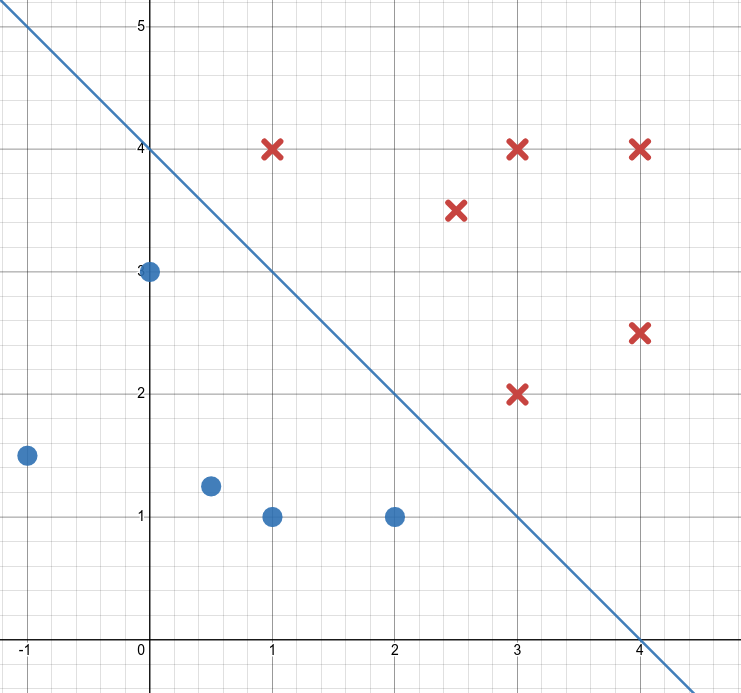
\includegraphics[align = c, width = \textwidth]{SVM-DesmosExample-WithLine}
		\begin{itemize}
			\item Blue circles: $y_i = -1$ 
			\item Red Xs: $y_i = 1$
			\item $-2 \sqrt 2 + \frac{\sqrt 2}{2} X_1 + \frac{\sqrt 2}{2} X_1 
			 = 0$
		\end{itemize}
		\column{.45\textwidth}
		\centering
		$y_i(\beta_0 + \beta_1 x_{i1} + \beta_2 x_{i2}) \geq M$
		
		\InstructorList{
			\item Ensures each on the correct side for a positive $M$
		  \item When we have unit normal coefficients, the second constraint is distance from the input point to the diagonal. 
		  \item Making sure every distance is bigger than $M$ and then make $M$ as big as possible
		}
		
	% Pushes the equation to the top when the instructor stuff isn't here
	\OnlyStudent{\vspace{2.3in}}
	
	
		\end{columns}
		\end{frame}
		%--- Next Frame ---%

		
\begin{frame}[t]{Mathematical Formulation}

	\begin{columns}
	\column{.65\textwidth}
	\centering
	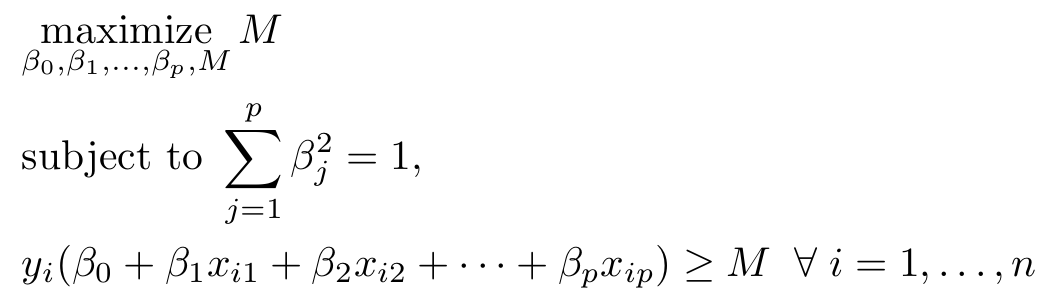
\includegraphics[width = \textwidth, align = c]{Eq9-9}
	\column{.35\textwidth}
	\centering
	\InstructorList{
		\item $M$ is making sure every point is at least distance $M$ from the hyperplane 
		\item Because of the $y_i$ multiplied, this also requires that the point is on the correct side of the hyperplane
	  \item Last eq forces points to be on the correct side of the hyperplane if $M>0$
		\item Making $M$ as big as possible is the maximal margin hyperplane
	}
	
	\end{columns}
	
	\end{frame}
	%--- Next Frame ---%
	%=================
	\section{Issues with Maximal Margin Classifier}
	%=================
	

\begin{frame}[t]{But what if....}

\begin{columns}
\column{.45\textwidth}
\centering
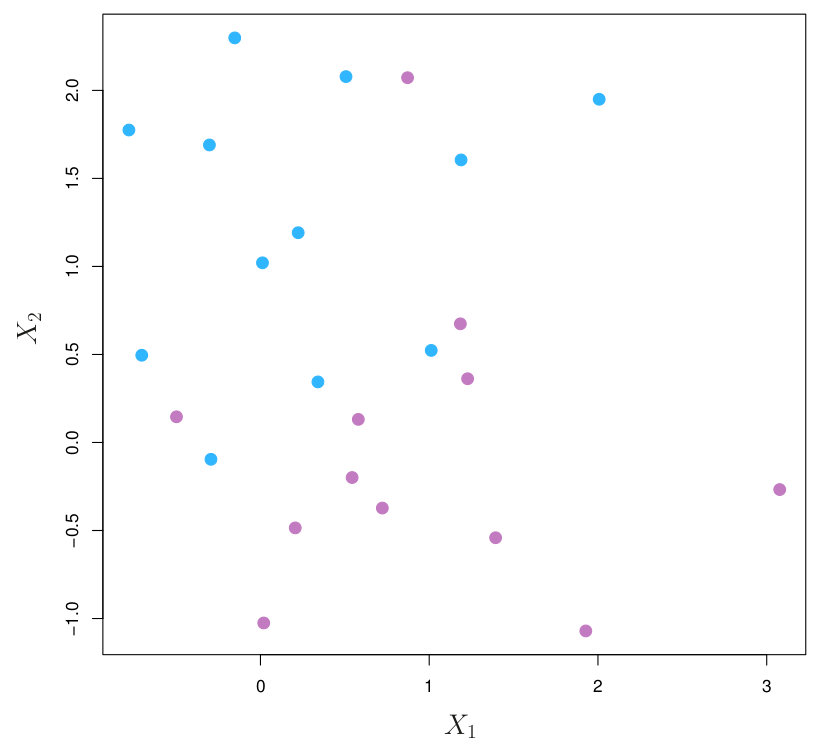
\includegraphics[width = \textwidth, align = c]{Fig9-4}
\column{.45\textwidth}
\centering
\InstructorList{
  \item
\InstructorNotes{...there is no separating hyperplane}
\item
\InstructorNotes{Means that there is no solution for $M>0$}
}


\end{columns}

\end{frame}
%--- Next Frame ---%

\begin{frame}[t]{Sensitivity to new points}
\InstructorNotes{Even if there is a spearating hyperplane might not be good}
\begin{columns}
\column{.4\textwidth}
\centering
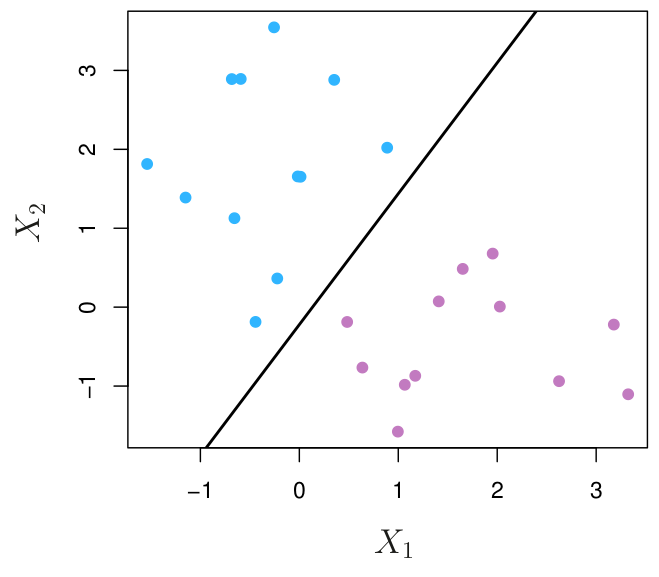
\includegraphics[width = \textwidth, align = c]{Fig9-5a}
\column{.4\textwidth}
\centering
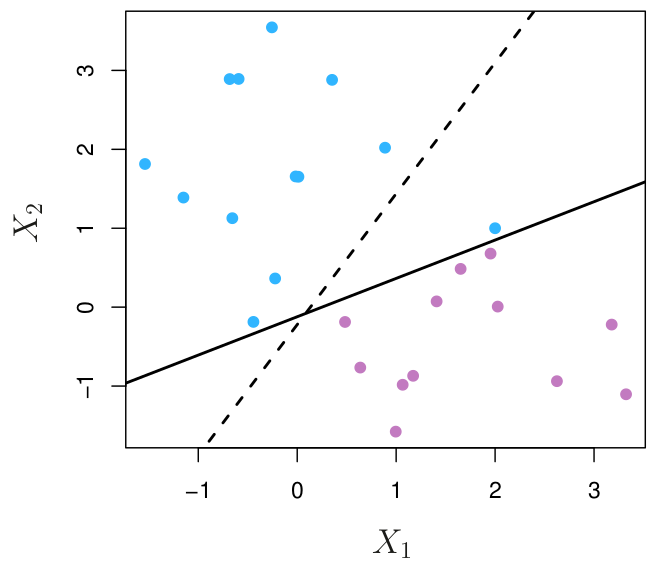
\includegraphics[width = \textwidth, align = c]{Fig9-5b}

\end{columns}
\footnotesize
\InstructorList{
  \item Add a blue observation on the right
	\item Dramatic shift in maximal margin hyperplane
}

\end{frame}
%--- Next Frame ---%


\begin{frame}[t]{Next time}
	\begin{columns}
		\column{.4\textwidth}
		\centering
		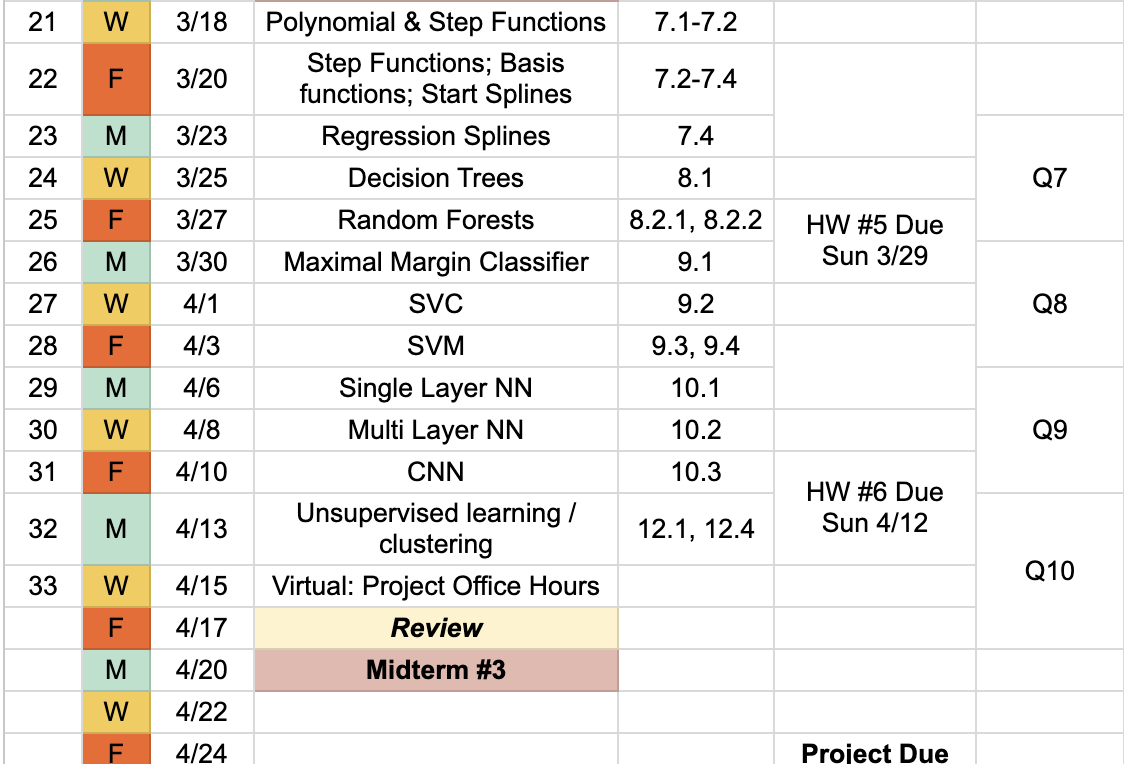
\includegraphics[align = l, width = \textwidth]{Schedule-S26-3.png}

		\column{.4\textwidth}
		% Q of the Day:

		% What is the relationship between ``support vectors'' and ``margin''?


		
	\end{columns}

\end{frame}
%--- Next Frame ---%


\end{document}
